\section{Increase in the number of critical paths}
\label{sec:criticalpaths}

The increased variance in delay caused by near-threshold operation is directly responsible for an increase in the number of critical paths.
A critical path can be defined as any path that has a high probability of exceeding a given clock~\cite{Wang:2004bw}.
For our case of trying to find the maximum frequency a given device can run, we can instead consider a critical path as a path that has a high probability of setting FMAX; that is, of being the slowest path in the system.
  
Consider a distribution of the nominal delays of paths within a process, in this case a synthesized ARM Cortex-M0 (Figure~\ref{fig:normal}).
In the case of no variations, clock speed is set by the path with the highest nominal delay (the nominal critical path).
Once delay variation is added in, however, paths that are close in delay to the nominal critical path could act instead as the critical path in a portion of chips.
This means that it is any path that falls within $n\frac{\sigma_v}{\mu}$ of the maximum nominal delay where $n$ is a constant that sets the guardband, $\sigma_v$ is the standard deviation, and $\mu$ is the mean of the timing path variation distribution.
The number of critical paths then becomes the area under this delay-count curve where the delay is greater than $n\frac{\sigma_v}{\mu}$
 
\begin{figure}[thpb]
    \centering
    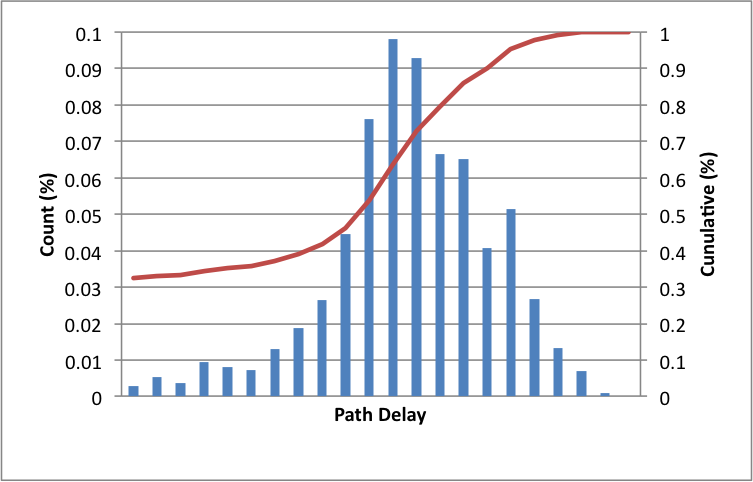
\includegraphics[width=0.4\textwidth]{pathlengths.png}
    \caption{Distribution of critical paths in a Cortex-M0. Path length increases to the right of the figure.}
    \label{fig:normal}
\end{figure}
 
Assuming the microcontroller was designed for $0.1\%$ of its paths to be critical, increasing $\frac{\sigma_v}{\mu}$ by 7x (as Dreslinski~\cite{Dreslinski:2010ez} suggests will happen in near-threshold) as the voltage drops into the near-threshold regime will cause this amount  to leap to $60\%$, an increase in the number of critical paths of 600x.

This vast increase in critical paths will translate into a reduction in the maximum frequency of the design. At the worst case, the overall chip slowdown scales as $1/\sqrt{n_{cp}}$ \cite{Bowman:2002cp}, which would in this case lead to a 24x slowdown.
